\begingroup
% Shared visual language for the three segmentation-method diagrams.
\tikzset{
    box/.style={draw, rounded corners=2pt, align=center, font=\small,
        text width=44mm, minimum height=9mm, inner sep=4pt, line width=0.5pt},
    process/.style={box, fill=gray!7},
    model/.style={box, very thick, fill=blue!5},
    output/.style={box, dashed},
    supervision/.style={box, densely dashed, fill=gray!7},
    link/.style={->, semithick},
    traininglink/.style={link, densely dashed}
}

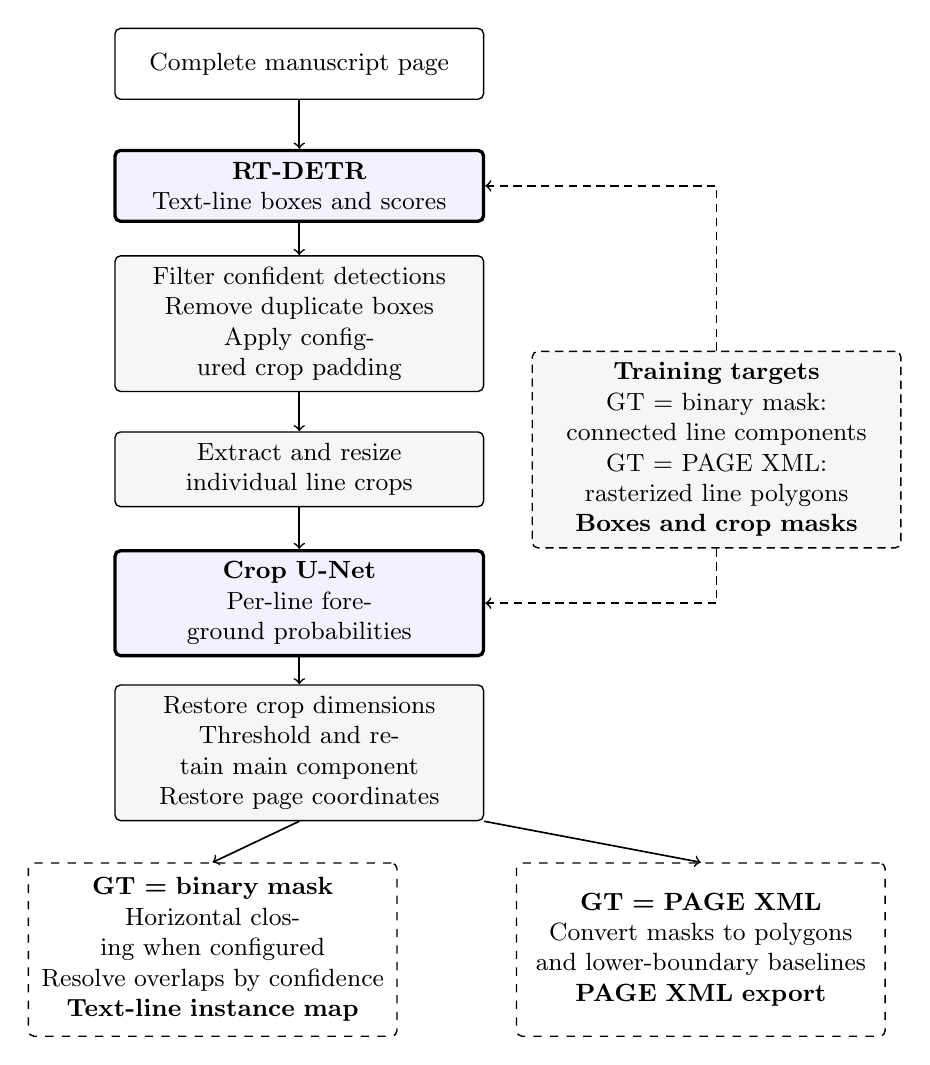
\begin{tikzpicture}
    \node[box] (page) at (-2,0) {Complete manuscript page};
    \node[model] (detector) at (-2,-1.55)
        {\textbf{RT-DETR}\\Text-line boxes and scores};
    \node[process] (boxes) at (-2,-3.3)
        {Filter confident detections\\Remove duplicate boxes\\Apply configured crop padding};
    \node[process] (crops) at (-2,-5.15)
        {Extract and resize\\individual line crops};
    \node[model] (segmenter) at (-2,-6.85)
        {\textbf{Crop U-Net}\\Per-line foreground probabilities};
    \node[process] (restore) at (-2,-8.75)
        {Restore crop dimensions\\Threshold and retain main component\\Restore page coordinates};
    \node[supervision] (targets) at (3.3,-4.9)
        {\textbf{Training targets}\\GT = binary mask:\\connected line components\\GT = PAGE XML:\\rasterized line polygons\\\textbf{Boxes and crop masks}};
    \node[output, minimum height=22mm] (binary-out) at (-3.1,-11.25)
        {\textbf{GT = binary mask}\\Horizontal closing when configured\\Resolve overlaps by confidence\\\textbf{Text-line instance map}};
    \node[output, minimum height=22mm] (xml-out) at (3.1,-11.25)
        {\textbf{GT = PAGE XML}\\Convert masks to polygons\\and lower-boundary baselines\\\textbf{PAGE XML export}};
    \draw[link] (page) -- (detector);
    \draw[link] (detector) -- (boxes);
    \draw[link] (boxes) -- (crops);
    \draw[link] (crops) -- (segmenter);
    \draw[link] (segmenter) -- (restore);
    \draw[link] (restore.south) -- (binary-out.north);
    \draw[link] (restore.south east) -- (xml-out.north);
    \draw[traininglink] (targets.north) |- (detector.east);
    \draw[traininglink] (targets.south) |- (segmenter.east);
\end{tikzpicture}
\endgroup
